\documentclass[aspectratio=169,11pt,t]{beamer}
% Beamer Preamble — Price Controls Cause Chaos
% Clean academic style

\usetheme{default}
\usecolortheme{default}

% ── Fonts ──
\usepackage{fontspec}
\defaultfontfeatures{Ligatures=TeX}
\setsansfont{Latin Modern Sans}
\setmonofont{Latin Modern Mono}

% ── Packages ──
\usepackage{amsmath,amssymb,amsthm}
\usepackage{graphicx}
\usepackage{booktabs}
\usepackage{tikz}
\usepackage{pgfplots}
\pgfplotsset{compat=1.18}
\usetikzlibrary{arrows.meta,calc,patterns,positioning,decorations.pathreplacing}
\usepackage{xcolor}
\usepackage{hyperref}
\usepackage{appendixnumberbeamer}

% ── Color Palette ──
\definecolor{GMUgreen}{RGB}{0,105,60}
\definecolor{GMUgold}{RGB}{185,154,52}
\definecolor{DarkSlate}{RGB}{52,73,94}
\definecolor{AlertRed}{RGB}{192,57,43}
\definecolor{SoftBlue}{RGB}{52,152,219}
\definecolor{LightGray}{RGB}{236,240,241}
\definecolor{MedGray}{RGB}{149,165,166}
\definecolor{DarkText}{RGB}{44,62,80}

% ── Beamer Structure Colors ──
\setbeamercolor{structure}{fg=DarkSlate}
\setbeamercolor{frametitle}{fg=DarkSlate,bg=white}
\setbeamercolor{title}{fg=DarkSlate}
\setbeamercolor{subtitle}{fg=MedGray}
\setbeamercolor{author}{fg=DarkText}
\setbeamercolor{date}{fg=MedGray}
\setbeamercolor{normal text}{fg=DarkText}
\setbeamercolor{alerted text}{fg=AlertRed}
\setbeamercolor{example text}{fg=GMUgreen}
\setbeamercolor{block title}{fg=white,bg=DarkSlate}
\setbeamercolor{block body}{bg=LightGray}
\setbeamercolor{block title alerted}{fg=white,bg=AlertRed}
\setbeamercolor{block body alerted}{bg=AlertRed!10}
\setbeamercolor{block title example}{fg=white,bg=GMUgreen}
\setbeamercolor{block body example}{bg=GMUgreen!8}
\setbeamercolor{itemize item}{fg=DarkSlate}
\setbeamercolor{itemize subitem}{fg=MedGray}
\setbeamercolor{footnote}{fg=MedGray}

% ── Beamer Fonts ──
\setbeamerfont{title}{size=\Large,series=\bfseries}
\setbeamerfont{frametitle}{size=\large,series=\bfseries}
\setbeamerfont{framesubtitle}{size=\small,series=\normalfont}
\setbeamerfont{author}{size=\normalsize}
\setbeamerfont{date}{size=\small}
\setbeamerfont{footnote}{size=\tiny}

% ── Beamer Templates ──
\setbeamertemplate{navigation symbols}{}
\setbeamertemplate{footline}{%
  \hfill\insertframenumber\,/\,\inserttotalframenumber\hspace{2mm}\vspace{2mm}%
}
\setbeamertemplate{frametitle}{%
  \vspace{4pt}%
  \insertframetitle%
  \ifx\insertframesubtitle\empty\else%
    \\[2pt]{\usebeamerfont{framesubtitle}\usebeamercolor[fg]{framesubtitle}\insertframesubtitle}%
  \fi%
  \vspace{-2pt}%
  {\color{GMUgold}\hrule height 0.8pt}%
  \vspace{4pt}%
}
\setbeamertemplate{itemize items}[circle]
\setbeamertemplate{enumerate items}[default]

% ── Custom Environments ──
\newenvironment{keybox}[1][Key Insight]{%
  \begin{beamercolorbox}[rounded=true,sep=6pt]{block title alerted}%
    \textbf{#1}%
  \end{beamercolorbox}%
  \begin{beamercolorbox}[rounded=true,sep=8pt]{block body alerted}%
}{%
  \end{beamercolorbox}%
}

\newenvironment{resultbox}[1][Result]{%
  \begin{beamercolorbox}[rounded=true,sep=6pt]{block title}%
    \textbf{#1}%
  \end{beamercolorbox}%
  \begin{beamercolorbox}[rounded=true,sep=8pt]{block body}%
}{%
  \end{beamercolorbox}%
}

\newenvironment{quoteslide}[1][]{%
  \begin{center}\large\itshape``%
}{%
  ''\end{center}%
}

% ── Shortcuts ──
\newcommand{\pbar}{\bar{p}}
\newcommand{\Qbar}{\bar{Q}}
\newcommand{\qbar}{\bar{q}}
\newcommand{\LMis}{L^{\text{Mis}}}
\newcommand{\LHarb}{L^{\text{Harb}}}
\newcommand{\emphcolor}[1]{{\color{AlertRed}\textbf{#1}}}
\newcommand{\goodcolor}[1]{{\color{GMUgreen}\textbf{#1}}}
\newcommand{\cmark}{\color{GMUgreen}\checkmark}
\newcommand{\xmark}{\color{AlertRed}\texttimes}


\graphicspath{{../Figures/extracted/}}

\title{Price Controls Cause Chaos}
\subtitle{Misallocation, Robust Bounds, and the 1973--74 Gasoline Crisis}
\author{Brian C.\ Albrecht \and Alex Tabarrok \and Mark Whitmeyer}
\institute{International Center for Law \& Economics \\ George Mason University \\ Arizona State University}
\date{February 2026}

\begin{document}

% ═══════════════════════════════════════════════════════════
% TITLE
% ═══════════════════════════════════════════════════════════

\begin{frame}[plain]
\titlepage
\end{frame}

% ═══════════════════════════════════════════════════════════
% PART I: MOTIVATION & PUZZLE
% ═══════════════════════════════════════════════════════════

\begin{frame}{February 1974}
\begin{columns}[T]
\column{0.55\textwidth}
\begin{itemize}
\item Aggregate gasoline shortfall: \emphcolor{$\approx 9\%$} nationwide
\item Price controls kept pump prices below market price
\item Textbook prediction: each market gets a proportional $\sim9\%$ reduction
\item Shadow prices equalize; Harberger triangle measures cost
\end{itemize}

\vspace{6pt}
\begin{keybox}[What actually happened?]
Not modest belt-tightening, but \emphcolor{feast or famine}.
\end{keybox}

\column{0.43\textwidth}
\vspace{6pt}
{\itshape\small ``Gasoline was in short supply in major urban areas, but there were more than abundant supplies in rural and vacation areas, where the only shortage was of tourists.''}

\vspace{4pt}
\hfill{\small --- Yergin (1991)}
\end{columns}
\end{frame}

\begin{frame}{The Patchwork of Rationing}
\begin{center}
\includegraphics[width=0.55\textwidth,trim=0 380 0 80,clip]{fig1_caption.png}
\end{center}
\vspace{-4pt}
{\footnotesize\textit{Percentage of stations rationing fuel by state, Feb 1974. Data: AAA surveys.}}
\end{frame}

\begin{frame}{The Puzzle}
\begin{columns}[T]
\column{0.48\textwidth}
\small
\textbf{Severe rationing:}
\begin{itemize}\setlength\itemsep{1pt}
\item Connecticut: $>90\%$ of stations
\item Massachusetts: $>90\%$
\item New Jersey, Rhode Island: $>60\%$
\end{itemize}

\vspace{4pt}
\textbf{No rationing at all:}
\begin{itemize}\setlength\itemsep{1pt}
\item Idaho, Montana, Utah, Wyoming: $0\%$
\item Hawaii: $0\%$
\end{itemize}

\column{0.48\textwidth}
\begin{keybox}[The overserved states are the problem]
\small
Under efficient allocation, a $9\%$ shortfall $\to$ proportional reduction \emph{everywhere}.

\vspace{3pt}
States with \emphcolor{zero rationing} were \emphcolor{overserved}: enough to satisfy demand even at the controlled price.
\end{keybox}
\end{columns}
\end{frame}

\begin{frame}{Reframing the Question}
\begin{center}
{\Large\bfseries The question is \emphcolor{not} why some states rationed.}

\vspace{8pt}
With a $9\%$ national shortfall, shortages somewhere are inevitable.

\vspace{16pt}
{\Large\bfseries The question is why other states exhibited \emphcolor{no rationing}.}

\vspace{8pt}
Why should some markets clear while others run dry?

\vspace{16pt}
\begin{resultbox}[Answer]
Efficient allocation requires \emph{price variation}. A binding ceiling explicitly forbids it.
\end{resultbox}
\end{center}
\end{frame}

\begin{frame}{This Paper: Three Contributions}
\begin{enumerate}
\item[\textbf{1.}] \textbf{The Chaos Theorem}\\[2pt]
Price controls generically produce corner allocations. Some markets get everything; others get nothing. Small parameter changes cause discontinuous jumps.

\vspace{6pt}
\item[\textbf{2.}] \textbf{Robust Bounds on Welfare}\\[2pt]
Sharp welfare bounds without assuming a demand functional form. Computation reduces to a 1D optimization.

\vspace{6pt}
\item[\textbf{3.}] \textbf{1973--74 Gasoline Crisis}\\[2pt]
Misallocation losses are \emphcolor{1--9$\times$ the Harberger triangle}. The quantity reduction is under $\frac{1}{3}$ of total welfare cost.
\end{enumerate}
\end{frame}

\begin{frame}{Roadmap}
\tableofcontents[hideallsubsections]
\end{frame}

% ═══════════════════════════════════════════════════════════
% PART II: TWO-MARKET EXAMPLE
% ═══════════════════════════════════════════════════════════

\section{Two-Market Intuition}

\begin{frame}{Setup: Two Submarkets}
\begin{itemize}
\item Two local markets with demands $D_1(p)$ and $D_2(p)$
\item Binding price ceiling $\pbar$ creates a total shortage:
\[
D(\pbar) - S(\pbar) > 0
\]
\item Total supply under the ceiling: $\Qbar \equiv S(\pbar)$
\item Feasible allocations: $q_1 + q_2 = \Qbar$, with $q_i \leq D_i(\pbar)$
\end{itemize}

\vspace{8pt}
\begin{resultbox}[Question]
How is $\Qbar$ split between the two markets?
\end{resultbox}
\end{frame}

\begin{frame}{Efficient vs.\ Corner Allocation}
\begin{center}
\includegraphics[height=0.82\textheight,trim=0 300 0 80,clip]{fig2_two_market.png}
\end{center}
\end{frame}

\begin{frame}{Panel A: The Harberger Benchmark}
\begin{columns}[T]
\column{0.55\textwidth}
\begin{itemize}
\item Shadow prices equalize across markets at $p^*$
\item Each market bears a proportional share of the shortage
\item Deadweight loss $=$ areas $a + b = c$ (the Harberger triangle)
\end{itemize}

\vspace{8pt}
This is what the textbook predicts.

\column{0.42\textwidth}
\begin{keybox}[But\ldots]
The Harberger triangle is not the \emph{average} outcome. It is the \emphcolor{minimum} welfare loss compatible with a binding ceiling.
\end{keybox}
\end{columns}
\end{frame}

\begin{frame}{Panel B: The Corner Allocation}
\begin{columns}[T]
\column{0.55\textwidth}
\begin{itemize}
\item Market 1 receives its full demand at $\pbar$
\item Market 2 gets whatever is left
\item Shadow prices \emphcolor{diverge}: Market 1 has low shadow price, Market 2 has very high shadow price
\item Welfare loss $a + b \gg c$
\end{itemize}

\vspace{8pt}
Nearly an order of magnitude larger than the Harberger triangle.

\column{0.42\textwidth}
\begin{keybox}[The geometry]
The constraint $q_1 + q_2 = \Qbar$ defines a \emph{line segment}. The endpoints $E_1$ and $E_2$ are corner solutions---and these are the generic equilibria.
\end{keybox}
\end{columns}
\end{frame}

\begin{frame}{The Feasible Set Is a Line Segment}
\begin{center}
\includegraphics[width=0.50\textwidth,trim=0 300 0 120,clip]{fig3_feasible_set.png}
\end{center}
{\footnotesize Corners $E_1$ and $E_2$ are the only generic equilibria. With costs $c_1 < c_2$, supply flows entirely to Market 1. Interior allocations are generically impossible.}
\end{frame}

\begin{frame}{Why Corners?}
\framesubtitle{The logic in four steps}

\begin{enumerate}
\item \textbf{Prices frozen} $\to$ sellers earn the same revenue everywhere
\item \textbf{Seller indifference} $\to$ allocation by \emph{cost minimization}
\item \textbf{Cost minimization is a linear program} on the feasible set
\item \textbf{Linear programs solve at corners}
\end{enumerate}

\vspace{8pt}
\begin{keybox}[The knife-edge]
Under market prices, a slight cost advantage for PA over NJ redirects \emph{a few tanker loads}.

Under price controls, it redirects \emphcolor{all of them}. A one-cent advantage is as good as one dollar.
\end{keybox}
\end{frame}

\begin{frame}{Prices vs.\ Price Controls: Incremental vs.\ Categorical}
\small
\begin{columns}[T]
\column{0.47\textwidth}
\begin{block}{Free Market}
\begin{itemize}\setlength\itemsep{2pt}
\item Arbitrage profits \emph{proportional} to price gap
\item Small cost advantage $\to$ small reallocation
\item Fine-grained, incremental adjustment
\end{itemize}
\end{block}

\column{0.47\textwidth}
\begin{alertblock}{Price Controls}
\begin{itemize}\setlength\itemsep{2pt}
\item Revenue equalized across destinations
\item Small cost advantage $\to$ \emphcolor{entire flow redirected}
\item All-or-nothing extremes
\end{itemize}
\end{alertblock}
\end{columns}

\vspace{8pt}
\begin{center}
\emph{The economy loses its capacity for incremental adjustment\\ and instead lurches between all-or-nothing extremes.}\\[2pt]
{\small --- Sowell (1980, p.\ 137)}
\end{center}
\end{frame}

% ═══════════════════════════════════════════════════════════
% PART III: GENERAL MODEL (Intuitive)
% ═══════════════════════════════════════════════════════════

\section{General Framework}

\begin{frame}{From Two Markets to Many}
\begin{itemize}
\item $n$ segmented submarkets; inverse demand $P_i(\cdot)$ in each
\item ``Submarket'' is deliberately flexible:
\begin{itemize}
\item Geographic: states, cities, countries
\item Temporal: summer vs.\ winter
\item Product: gasoline vs.\ diesel vs.\ heating oil
\item Production stage: crude $\to$ refined products
\end{itemize}
\item A binding ceiling $\pbar$ fixes total supply at $\Qbar = S(\pbar)$
\end{itemize}

\vspace{8pt}
\textbf{Feasible set:}
\[
\mathcal{F} = \left\{ q \in \mathbb{R}_+^n : \sum_{i=1}^n q_i = \Qbar,\; 0 \leq q_i \leq \qbar_i \;\forall\, i \right\}
\]

A convex polytope. Its \emphcolor{vertices} have $q_i \in \{0, \qbar_i\}$ for all but at most one market.
\end{frame}

\begin{frame}{Welfare and Misallocation}
\textbf{Consumer surplus} in market $i$ at allocation $q_i$:
\[
W_i(q_i) = \int_0^{q_i} \bigl[P_i(x) - \pbar\bigr]\, dx
\]

\vspace{4pt}
\textbf{Efficient allocation} $q^*$: equalize shadow prices across all served markets.

\vspace{8pt}
\begin{resultbox}[Misallocation Deadweight Loss]
\[
\LMis(q) = W(q^*) - W(q) = \sum_{i=1}^n \int_{q_i}^{q_i^*} P_i(x)\, dx
\]
The welfare destroyed by distributing the fixed supply $\Qbar$ inefficiently. These are the \emph{dollars left on the table} when goods don't flow to their highest-value uses.
\end{resultbox}
\end{frame}

\begin{frame}{Worst-Case Allocations}
\begin{resultbox}[Theorem 1 (Worst Case)]
The worst-case allocation---the one that \emph{maximizes} deadweight loss---sits at a \textbf{vertex} of $\mathcal{F}$:
\[
q_i \in \{0, \qbar_i\} \quad \text{for all but at most one market}
\]
\end{resultbox}

\vspace{8pt}
\textbf{Intuition:}
\begin{itemize}
\item Welfare (gross surplus) is concave $\to$ its minimum is at an extreme point
\item The worst case concentrates supply in markets where it generates the \emph{least} value
\item Markets with high choke prices receive nothing; markets with low shadow prices are flooded
\end{itemize}

\vspace{8pt}
There exists a cutoff $\lambda$: markets with $P_i(0) \geq \lambda$ get nothing; those with $P_i(\qbar_i) \leq \lambda$ get everything.
\end{frame}

% ═══════════════════════════════════════════════════════════
% PART IV: THE CHAOS THEOREM
% ═══════════════════════════════════════════════════════════

\section{The Chaos Theorem}

\begin{frame}{Without Price Controls: Smooth Markets}
\begin{itemize}
\item Parameters $\theta$ govern demands $P_i(x;\theta)$, costs $c_i(\theta)$, supply $\Qbar(\theta)$
\item Under free markets, the allocation that maximizes surplus is:
\[
q^*(\theta) = \arg\max_{q \geq 0} \left\{ \sum_i \int_0^{q_i} P_i(x;\theta)\,dx - \sum_i c_i(\theta) q_i \right\}
\quad \text{s.t.}\;\sum_i q_i = \Qbar(\theta)
\]
\item Objective is strictly concave $\Rightarrow$ unique $q^*(\theta)$
\item By Berge's Maximum Theorem: $q^*(\theta)$ is \goodcolor{continuous} in $\theta$
\end{itemize}

\vspace{8pt}
\begin{exampleblock}{}
\textbf{Small changes in parameters $\to$ small changes in allocations and welfare.}
\end{exampleblock}
\end{frame}

\begin{frame}{Under Price Controls: Cost Minimization}
Now impose a binding ceiling $\pbar$. All units sell at $\pbar$, so profit-maximizing suppliers \emphcolor{minimize delivery costs}:
\[
\min_{q \in \mathcal{F}(\theta)} \; c(\theta) \cdot q
\]

\vspace{8pt}
This is a \textbf{linear program}. With generically distinct costs:
\begin{itemize}
\item Markets are filled in order of \emph{increasing cost}
\item At most one market is partially filled
\item When two markets have nearly equal costs, an infinitesimal change can \emphcolor{flip the entire allocation}
\end{itemize}

\vspace{8pt}
\begin{alertblock}{}
The equilibrium allocation becomes \textbf{discontinuous} in parameters.
\end{alertblock}
\end{frame}

\begin{frame}{The Chaos Theorem}
\begin{resultbox}[Theorem 2 (Chaos)]
Suppose two adjacent vertex allocations $v$ and $w$ are both optimal at some parameter $\theta^*$. If the welfare difference $\Delta W \neq 0$ (a generic condition), then for every neighborhood of $\theta^*$:

\vspace{6pt}
\begin{enumerate}
\item The optimal allocation \emphcolor{jumps discontinuously} between $v$ and $w$
\item Welfare jumps by $+|\Delta W|$ along one path and $-|\Delta W|$ along another
\end{enumerate}

\vspace{6pt}
Welfare is \textbf{not locally monotone}: arbitrarily small perturbations can move welfare up or down by discrete amounts.
\end{resultbox}

\vspace{6pt}
A pipeline repair, a regulatory tweak, a refinery outage---\emph{any} small change in relative costs can flip the entire allocation, with potentially catastrophic welfare consequences.
\end{frame}

\begin{frame}{The Chaos of Price Controls: Intuition}
\begin{center}
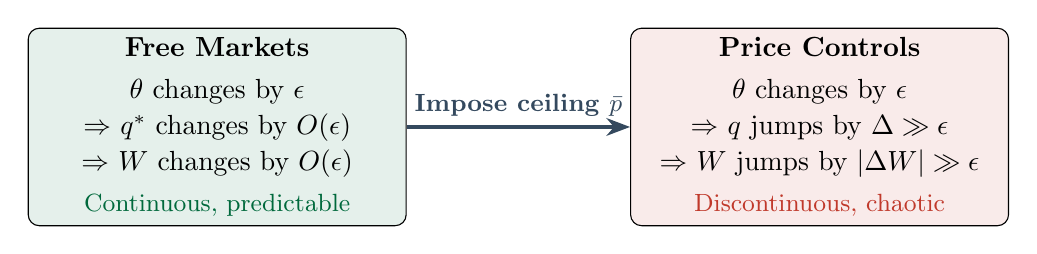
\begin{tikzpicture}[scale=0.85]
\node[draw, rounded corners, fill=GMUgreen!10, minimum width=4.8cm, minimum height=2.5cm, align=center] (fm) at (-4.5,0) {
\textbf{Free Markets}\\[3pt]
$\theta$ changes by $\epsilon$\\[1pt]
$\Rightarrow$ $q^*$ changes by $O(\epsilon)$\\[1pt]
$\Rightarrow$ $W$ changes by $O(\epsilon)$\\[3pt]
{\small\color{GMUgreen} Continuous, predictable}
};
\node[draw, rounded corners, fill=AlertRed!10, minimum width=4.8cm, minimum height=2.5cm, align=center] (pc) at (4.5,0) {
\textbf{Price Controls}\\[3pt]
$\theta$ changes by $\epsilon$\\[1pt]
$\Rightarrow$ $q$ jumps by $\Delta \gg \epsilon$\\[1pt]
$\Rightarrow$ $W$ jumps by $|\Delta W| \gg \epsilon$\\[3pt]
{\small\color{AlertRed} Discontinuous, chaotic}
};
\draw[-{Stealth[length=3mm]}, very thick, DarkSlate] (fm.east) -- (pc.west) node[midway,above,font=\small\bfseries] {Impose ceiling $\pbar$};
\end{tikzpicture}
\end{center}

\vspace{4pt}
\begin{center}
\emph{Price controls introduce fundamental unpredictability.\\ Allocations become hypersensitive to ``nuisance parameters''\\ that would be irrelevant under market clearing.}
\end{center}
\end{frame}

\begin{frame}{Simulation: 100 Markets on a Grid}
\framesubtitle{Three random cost draws; free market (top) vs.\ price controls (bottom)}
\begin{center}
\includegraphics[height=0.80\textheight,trim=0 300 0 60,clip]{fig4_simulation.png}
\end{center}
\end{frame}

\begin{frame}{What the Simulation Shows}
\begin{enumerate}
\item \textbf{Free-market allocations are nearly identical} across scenarios---small cost differences $\to$ small allocation differences

\vspace{4pt}
\item \textbf{Under price controls, many markets receive zero} (yellow)---low-cost cities fill to capacity; $\sim30$ cities get nothing

\vspace{4pt}
\item \textbf{Different cost draws $\to$ radically different allocations}---same demand, same supply, completely different spatial pattern
\end{enumerate}

\vspace{6pt}
\begin{keybox}[This is the Chaos Theorem in action]
Small changes in nuisance parameters dramatically change the allocation. Welfare loss: $\sim 13\%$.
\end{keybox}
\end{frame}

% ═══════════════════════════════════════════════════════════
% PART V: ROBUST BOUNDS
% ═══════════════════════════════════════════════════════════

\section{Robust Bounds on Welfare}

\begin{frame}{The Identification Problem}
\small
\begin{itemize}\setlength\itemsep{2pt}
\item Chaos Theorem $\Rightarrow$ expect \emphcolor{corner allocations}---far from market equilibria
\item Welfare depends on values at these extreme quantities
\item But demand is identified only \emph{locally}, near equilibrium
\end{itemize}

\vspace{4pt}
\begin{columns}[T]
\column{0.55\textwidth}
\textbf{The extrapolation problem:}
\begin{itemize}\setlength\itemsep{1pt}
\item Closed stations: $\sim 67\%$ of baseline
\item Elasticity estimates: near $q = 1$, not $q = 0.67$
\item From $\varepsilon = 0.2$: $P(0) = 6$
\item From $\varepsilon = 0.4$: $P(0) = 3.5$
\item Welfare difference: $4\%$ vs.\ $16\%$ of baseline
\end{itemize}

\column{0.42\textwidth}
\begin{keybox}[Our approach]
\small
No parametric demand assumption.

\vspace{3pt}
Largest and smallest welfare losses consistent with:
\begin{itemize}\setlength\itemsep{1pt}
\item Observed allocations
\item Slope bounds (from elasticity)
\item A finite choke price
\end{itemize}
\end{keybox}
\end{columns}
\end{frame}

\begin{frame}{Step 1: Slope Bounds Create a ``Wedge''}
\framesubtitle{What we know constrains what demand can look like}

\begin{columns}[T]
\column{0.55\textwidth}
\textbf{Assumptions:}
\begin{itemize}
\item Observe anchor point $(q_i^{\text{obs}}, p_{0,i})$ on each demand curve
\item Slope bounds: $g_{i,L} \leq P_i'(q) \leq g_{i,U} < 0$
\item Choke bound: $P_i(0) \leq M_i$
\end{itemize}

\vspace{8pt}
The slope bounds force $P_i$ to lie in a \textbf{wedge}---between rays with slopes $g_{i,L}$ (steep) and $g_{i,U}$ (flat) emanating from the anchor.

\column{0.42\textwidth}
\begin{center}
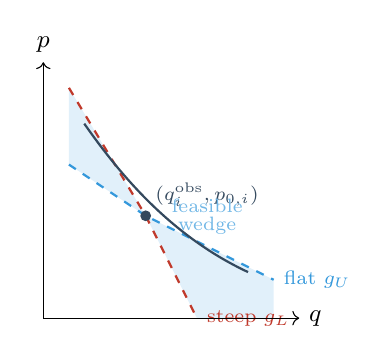
\begin{tikzpicture}[scale=0.65]
\fill[SoftBlue!15] (0.5,4.5) -- (2,2) -- (4.5,0.75) -- (4.5,0) -- (3,0) -- (2,2) -- (0.5,3) -- cycle;
\draw[thick, AlertRed, dashed] (0.5,4.5) -- (2,2) -- (3,0) node[right, font=\scriptsize] {steep $g_L$};
\draw[thick, SoftBlue, dashed] (0.5,3) -- (2,2) -- (4.5,0.75) node[right, font=\scriptsize] {flat $g_U$};
\draw[thick, DarkSlate] (0.8,3.8) .. controls (1.5,2.8) and (2.5,1.6) .. (4,0.9);
\fill[DarkSlate] (2,2) circle (3pt) node[above right, font=\scriptsize] {$(q_i^{\text{obs}}, p_{0,i})$};
\draw[->] (0,0) -- (5,0) node[right] {\small $q$};
\draw[->] (0,0) -- (0,5) node[above] {\small $p$};
\node[font=\scriptsize, SoftBlue!70] at (3.2,2.2) {feasible};
\node[font=\scriptsize, SoftBlue!70] at (3.2,1.8) {wedge};
\end{tikzpicture}
\end{center}
\end{columns}
\end{frame}

\begin{frame}{Step 2: Invert the Wedge $\to$ Quantity Bands}
\begin{columns}[T]
\column{0.55\textwidth}
\begin{itemize}
\item At each price $p$, the feasible quantity lies in a band:
\[
\ell_i(p) \leq q_i(p) \leq u_i(p)
\]
\item The wedge in $(q,p)$ space becomes pointwise box constraints in $(p,q)$ space
\end{itemize}

\vspace{8pt}
\textbf{Step 3: Feasible shadow prices}
\begin{itemize}
\item Define $L(p) = \sum_i \ell_i(p)$, $U(p) = \sum_i u_i(p)$
\item A shadow price $p$ is feasible iff:
\[
\mathcal{I} = \{p : L(p) \leq \Qbar \leq U(p)\}
\]
\end{itemize}

\column{0.42\textwidth}
\begin{center}
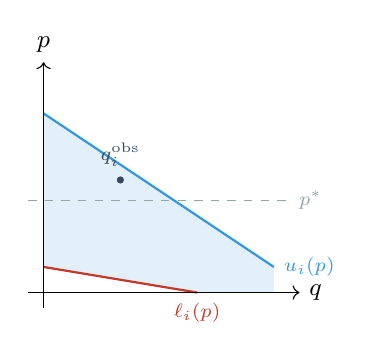
\begin{tikzpicture}[scale=0.65]
% Band illustration
\fill[SoftBlue!15] (0,0.5) -- (0,3.5) -- (4.5,0.5) -- (4.5,0) -- (3,0) -- cycle;
\draw[thick, SoftBlue] (0,3.5) -- (4.5,0.5) node[right, font=\scriptsize] {$u_i(p)$};
\draw[thick, AlertRed] (0,0.5) -- (3,0) node[below, font=\scriptsize] {$\ell_i(p)$};
\draw[dashed, MedGray] (-0.3,1.8) -- (4.8,1.8) node[right, font=\scriptsize] {$p^*$};
\fill[DarkSlate] (1.5,2.2) circle (2pt);
\node[font=\scriptsize, DarkSlate] at (1.5,2.7) {$q_i^{\text{obs}}$};
\draw[->] (0,-0.3) -- (0,4.5) node[above] {\small $p$};
\draw[->] (-0.3,0) -- (5,0) node[right] {\small $q$};
\end{tikzpicture}
\end{center}
\end{columns}
\end{frame}

\begin{frame}{Step 4: One-Dimensional Optimization}
\framesubtitle{The heart of the approach}
\small
\textbf{Key identity} (welfare gap in price space):
\[
\Phi(P) = \Qbar p^* - \sum_i q_i^{\text{obs}} p_{0,i} - \sum_i \int_{p_{0,i}}^{p^*} q_i(p)\, dp
\]

\begin{resultbox}[Lemma 1 (Reduction to 1D)]
\small
Objective is \textbf{linear} in $q_i(\cdot)$; constraints are boxes $q_i(p) \in [\ell_i(p), u_i(p)]$.

$\Rightarrow$ Worst/best cases push $q_i$ to \emphcolor{endpoints}. $\overline{\Phi}(p)$ and $\underline{\Phi}(p)$ become \textbf{scalar functions of $p \in \mathcal{I}$}.
\end{resultbox}

\vspace{4pt}
\textbf{Theorem 3:} Sharp bounds attained by \emph{piecewise-linear} demands with slopes $\in \{g_L, g_U\}$. Not sensitivity analysis---exact over \emph{all} Lipschitz functions satisfying slope constraints.
\end{frame}

% ═══════════════════════════════════════════════════════════
% PART VI: EMPIRICAL APPLICATION
% ═══════════════════════════════════════════════════════════

\section{The 1973--74 Gasoline Crisis}

\begin{frame}{Historical Context}
\begin{itemize}
\item \textbf{August 1971:} Nixon freezes all wages and prices
\item Petroleum remains under controls even after other prices unfrozen
\item \textbf{August 1973:} Special Rule No.\ 1 --- mandatory petroleum controls
\item \textbf{October 1973:} Oil Embargo begins; market price triples
\item Controls + embargo = severe shortages
\item \textbf{EPAA (1973):} Allocation system based pro-rata on 1972 levels
\begin{itemize}
\item If supply falls to 90\% of 1972, each buyer gets 90\% of 1972 allocation
\item Plus exceptions for defense, agriculture, essential services\ldots
\item All under an ``equitable'' guideline
\end{itemize}
\end{itemize}

\vspace{6pt}
\begin{keybox}
Despite pro-rata rules, the outcome was \emphcolor{extreme dispersion}---exactly what the Chaos Theorem predicts.
\end{keybox}
\end{frame}

\begin{frame}{The Data: AAA Station Surveys, February 1974}
\begin{columns}[T]
\column{0.48\textwidth}
\textbf{Station-level classification:}
\begin{itemize}
\item $10.1\%$ of stations: \emphcolor{closed} (out of fuel)
\item $27.8\%$: \emphcolor{limiting purchases}
\item $62.1\%$: operating normally
\end{itemize}

\vspace{8pt}
Mean out-of-fuel rate by state: $8.2\%$

But this average masks \emph{striking heterogeneity}

\column{0.48\textwidth}
\textbf{Our aggregation:}
\begin{itemize}
\item Two markets: \textbf{Open} (62\%) vs.\ \textbf{Closed/Limiting} (38\%)
\item Open stations: $q_O = 1.06$ (demand at $\pbar$)
\item Closed/limiting: $q_C \approx 0.67$ (residual)
\end{itemize}

\vspace{8pt}
This is the corner-solution structure predicted by the Chaos Theorem.
\end{columns}
\end{frame}

\begin{frame}{Welfare Measures}
\textbf{Harberger deadweight loss} (quantity reduction, efficient allocation):
\[
\LHarb = \widetilde{W}(q^{\text{base}}) - \widetilde{W}(q^*) - \pbar \cdot (Q^{\text{base}} - \Qbar) \approx 2.03\%
\]

\textbf{Misallocation loss} (inefficient distribution of reduced supply):
\[
\LMis = W(q^*) - W(q^{\text{obs}})
\]

\vspace{8pt}
\begin{resultbox}[Misallocation Ratio]
\[
R = \frac{\LMis}{\LHarb}
\]
$R = 0$: efficient rationing. \quad $R = 1$: misallocation doubles the cost. \quad $R > 1$: misallocation \emphcolor{dominates}.
\end{resultbox}

\vspace{4pt}
All losses expressed as \% of baseline expenditure ($p_{\text{base}} \times Q_{\text{base}}$).
\end{frame}

\begin{frame}{Station-Level Demand Curves (No Choke Constraint)}
\begin{center}
\includegraphics[height=0.75\textheight,trim=0 120 0 80,clip]{fig5_station_demand_no_choke.png}
\end{center}
\end{frame}

\begin{frame}{Station-Level Demand Curves (With Choke $M = 4$)}
\begin{center}
\includegraphics[height=0.75\textheight,trim=0 120 0 80,clip]{fig6_station_demand_choke.png}
\end{center}
\end{frame}

\begin{frame}{Shadow Price Ranges}
\begin{center}
\includegraphics[height=0.65\textheight,trim=0 100 0 100,clip]{fig7_shadow_price_ranges.png}
\end{center}
{\footnotesize Blue: no-choke ranges. Orange: with choke $P(0) \leq M = 4$. Choke tightens closed/limiting upper bound.}
\end{frame}

\begin{frame}{Station-Level Results}
\small
\begin{columns}[T]
\column{0.55\textwidth}
At baseline ($\pbar = 0.8$, $\varepsilon \in [0.2, 0.4]$):

\vspace{4pt}
\begin{keybox}[Headline Result]
\small
\vspace{-4pt}
\[
\frac{\LMis}{\LHarb} \in [1.13,\; 9.06]
\]
\vspace{-6pt}
Misallocation loss: $[2.29\%, 18.36\%]$ of baseline spending. With choke $M = 4$: upper $\to 6.23$.
\end{keybox}

\vspace{4pt}
Harberger triangle ($\approx 2\%$): less than $\frac{1}{3}$ of total welfare cost.

\column{0.42\textwidth}
\textbf{Sensitivity to $\pbar$:}

\vspace{4pt}
\begin{tabular}{cc}
\toprule
$\pbar$ & $R$ interval \\
\midrule
0.5 & $[2.90, 23.20]$ \\
\textbf{0.8} & $\mathbf{[1.13, 9.06]}$ \\
1.0 & $[0.41, 3.26]$ \\
\bottomrule
\end{tabular}

\vspace{6pt}
Deeper controls $\to$ wider interval, higher upper bound.
\end{columns}
\end{frame}

\begin{frame}{State-Level Analysis: 48 Markets}
\small
\begin{columns}[T]
\column{0.55\textwidth}
\textbf{Why disaggregate to states?}
\begin{itemize}\setlength\itemsep{1pt}
\item Adding-up $\sum_i q_i = \Qbar$ genuinely binds across 48 markets
\item Giving more to CT means taking from CA
\item This \emph{disciplines} the bounds
\end{itemize}

\vspace{4pt}
\begin{resultbox}[State-Level Result]
\small
\vspace{-4pt}
\[
\frac{\LMis}{\LHarb} \in [0.26,\; 2.38]
\]
\vspace{-6pt}
Tighter: adding-up discipline + assumes efficient within-state allocation.
\end{resultbox}

\column{0.42\textwidth}
\begin{keybox}[The gap between levels]
\small
Station-level: \emphcolor{total} misallocation (across + within states)

\vspace{2pt}
State-level: only \emph{across-state}

\vspace{2pt}
CT's 90\% $\to$ one average, obscuring open vs.\ closed within CT.
\end{keybox}
\end{columns}
\end{frame}

\begin{frame}{State Shadow-Price Bounds}
\begin{center}
\includegraphics[height=0.72\textheight,trim=0 120 0 80,clip]{fig8_state_shadow_prices.png}
\end{center}
{\footnotesize Red = higher shadow prices; blue = lower. High-rationing states in red.}
\end{frame}

\begin{frame}{State-Level Shadow Prices by State}
\begin{center}
\includegraphics[height=0.80\textheight,trim=0 40 0 40,clip]{fig9_state_bounds_by_state.png}
\end{center}
\end{frame}

% ═══════════════════════════════════════════════════════════
% PART VII: BEYOND GEOGRAPHY
% ═══════════════════════════════════════════════════════════

\section{Misallocation Beyond Geography}

\begin{frame}{The Chaos Mechanism Is General}
\framesubtitle{Same logic whenever controls suppress price variation across segments}
\small
\begin{columns}[T]
\column{0.48\textwidth}
\textbf{Product-mix misallocation:}
\begin{itemize}\setlength\itemsep{1pt}
\item A barrel of crude $\to$ gasoline, diesel, heating oil, jet fuel\ldots
\item Controlled prices + small cost wedges $\to$ large shifts in fuel mix
\item Shortages rotated unpredictably across fuels
\end{itemize}

\column{0.48\textwidth}
\textbf{Temporal misallocation:}
\begin{itemize}\setlength\itemsep{1pt}
\item Heating oil prices frozen at \emph{summer 1971} levels
\item Weakened incentives to store for winter
\item Winter shortages, school closures
\item ``Freezing prices led to freezing people''
\end{itemize}
\end{columns}

\vspace{6pt}
\begin{center}
{\small\emph{``Phases 3 and 3A have created price anomalies that frequently prevent the movement of products in proper directions.''} --- 1973 Congressional testimony}
\end{center}
\end{frame}

\begin{frame}{The Baby Chicks}
\framesubtitle{Input--output misallocation under price controls}
\small
\begin{columns}[T]
\column{0.55\textwidth}

In summer 1973, chicken farmers \emphcolor{gassed, drowned, and suffocated roughly one million baby chicks}.

\vspace{4pt}
\textbf{The mechanism:}
\begin{itemize}\setlength\itemsep{1pt}
\item Retail chicken prices: \emphcolor{controlled}
\item Feed costs: \emph{not controlled}
\item Revenue capped along the grow-out path
\item Small feed-cost increases $\to$ abandon ``raise chicks'' segment entirely
\end{itemize}

\vspace{4pt}
{\itshape ``It's cheaper to drown 'em than to put 'em down and raise 'em.''}\\
\hfill{\scriptsize --- AP, 1973}

\column{0.42\textwidth}
\textbf{Same pattern elsewhere:}
\begin{itemize}\setlength\itemsep{1pt}
\item Dairy farmers slaughtered cows
\item Hog farmers culled breeding stock
\item Temporarily $\uparrow$ meat, future $\downarrow$
\end{itemize}

\vspace{4pt}
\begin{keybox}[Corner solution]
\small
Controls flattened returns across time.

Small cost wedges $\to$ \emphcolor{vertex}: all supply to ``now,'' zero to ``later.''
\end{keybox}
\end{columns}
\end{frame}

\begin{frame}{Supply-Chain Amplification}
\small
\begin{itemize}\setlength\itemsep{2pt}
\item Allocation rules designated priority end uses
\item But policymakers \emphcolor{underestimated input--output linkages}
\end{itemize}

\vspace{4pt}
\textbf{Example: Propane $\to$ plastic pipe $\to$ oil wells}
\begin{itemize}\setlength\itemsep{1pt}
\item Oil production was prioritized
\item Propane: essential for plastic piping used in oil extraction
\item Plastics industry initially \emph{lacked} priority designation
\item Pipe shortages disrupted the very oil production that policy sought to protect
\end{itemize}

\vspace{4pt}
\begin{keybox}[Price controls metastasize]
\small
Shortage-chaos $\to$ demand for quantity management $\to$ yield regulations, inventory mandates, bureaucratic allocation. Once prices can't do their job, ``the market'' delivers \emphcolor{corner outcomes with no welfare ordering}.
\end{keybox}
\end{frame}

% ═══════════════════════════════════════════════════════════
% PART VIII: CONCLUSION
% ═══════════════════════════════════════════════════════════

\section{Conclusion}

\begin{frame}{Summary of Results}
\begin{enumerate}
\item[\textbf{1.}] \textbf{Chaos Theorem:} Under price controls, equilibrium generically lands at \emphcolor{corners} where some markets are fully served and others get nothing. Small parameter changes cause discontinuous jumps.

\vspace{8pt}
\item[\textbf{2.}] \textbf{Robust Bounds:} Without assuming a demand functional form, misallocation losses can be bounded using only observed allocations, slope bounds, and a choke price. Sharp bounds are attained by piecewise-linear demands.

\vspace{8pt}
\item[\textbf{3.}] \textbf{Empirical Evidence:} In the 1973--74 gasoline crisis, misallocation losses were \emphcolor{1--9$\times$ the Harberger triangle}. The quantity reduction accounts for under one-third of total welfare cost.
\end{enumerate}
\end{frame}

\begin{frame}{The Broader Lesson}
\begin{center}

\vspace{24pt}
{\Large\itshape Whenever a ceiling fragments an integrated market---\\[6pt]
gasoline, rental housing, agriculture, medical care---\\[6pt]
the main cost is not the familiar triangle,\\[6pt]
but the \emphcolor{hidden misallocation} behind it.}

\vspace{36pt}
{\large Thank you.}
\end{center}
\end{frame}

\end{document}
